\subsection{Les filtres}

\begin{frame}{Utilité}
    \begin{block}{Explication}
        % Les filtres sont utilisés pour améliorer la qualité des mesures issues des capteurs avant qu'elles ne soient exploitées par le contrôleur. Les mesures réelles sont en effet sont pertrubées par du bruit, des parasites ou des variations rapides qui peuvent dégrader les performances d'un système asservi.
        
        \begin{itemize}
            \item Filtrer les mesures des capteurs.
            \item Atténuer le bruit et les perturbations.
            \item Améliorer les performances du système asservi.
        \end{itemize}
    \end{block}
    
    \begin{block}{Exploitation}
        % Il existe différents type de filtres, ceux qu'on va expérimenter sont les filtres passe-bas et passe-haut, le premier permet d'atténuer les hautes fréquences et le deuxième les basses fréquences. Coupler ensemble cela devient un passe bande qui permet d'atténuer les fréquences qui ne sont pas entre les deux intervalles.
        
        \begin{itemize}
            \item Expérimenter les filtres passe-bas et passe-haut.
            \item Atténuer les hautes ou les basses fréquences.
            \item Combiner les filtres pour obtenir un passe-bande.
        \end{itemize}
    \end{block}
\end{frame}

\begin{frame}{Passe-bas et passe-haut (Butterworth ordre 2)}

\vspace{5mm}

\begin{block}{Contexte}
    % Le filtre de Butterworth a été proposé par Stephen Butterworth en 1930 afin d'obtenir une réponse fréquentiellement maximalement plate dans la bande passante. Ce qui signifie qu'on va préserver les informations utiles du signal tout en améliorant fortement l'atténuation des hautes ou basses fréquences
    
    \begin{itemize}
        \item Choisir un filtre de Butterworth.
        \item Préserver les informations utiles du signal.
        \item Atténuer efficacement les fréquences indésirables.
    \end{itemize}
\end{block}

\vspace{-2mm}

    \begin{block}{Equation}
    $$y_{n} = b_{0}x_{n} + b_{1}x_{n-1} + b_{2}x_{n-2} - a_{1}y_{n-1} - a_{2}y_{n-2}$$
    où :
    \begin{itemize}
        \item $y_{n}$ : la sortie à l'instant n.
        \item $x_{n}$ : l'entrée à l'instant n.
        \item $a_{1,2}$ et $b_{0,1,2}$ : des variables a définir.
    \end{itemize}
    \end{block}
\end{frame}

\begin{frame}{Exemple musical}
    \begin{block}{Contexte}
\begin{itemize}
    \item On utilise un fichier audio mixé qui contient comme instrument une basse, une guitare électrique et une flûte tous ayant des fréquences différentes.
    \item Basse : 30 Hz à 250 Hz.
    \item Guitare électrique : 280 Hz à 900 Hz.
    \item Flûte : 1000 Hz à 1400 Hz.
\end{itemize}
    \end{block}
    
    \begin{block}{Objectif}
        Filtrer ces données pour obtenir seulement le signal de la basse.
    \end{block}
\end{frame}

\begin{frame}{Résultats - Spectre fréquentiel de la piste audio de la basse}

\begin{figure}
    \centering
    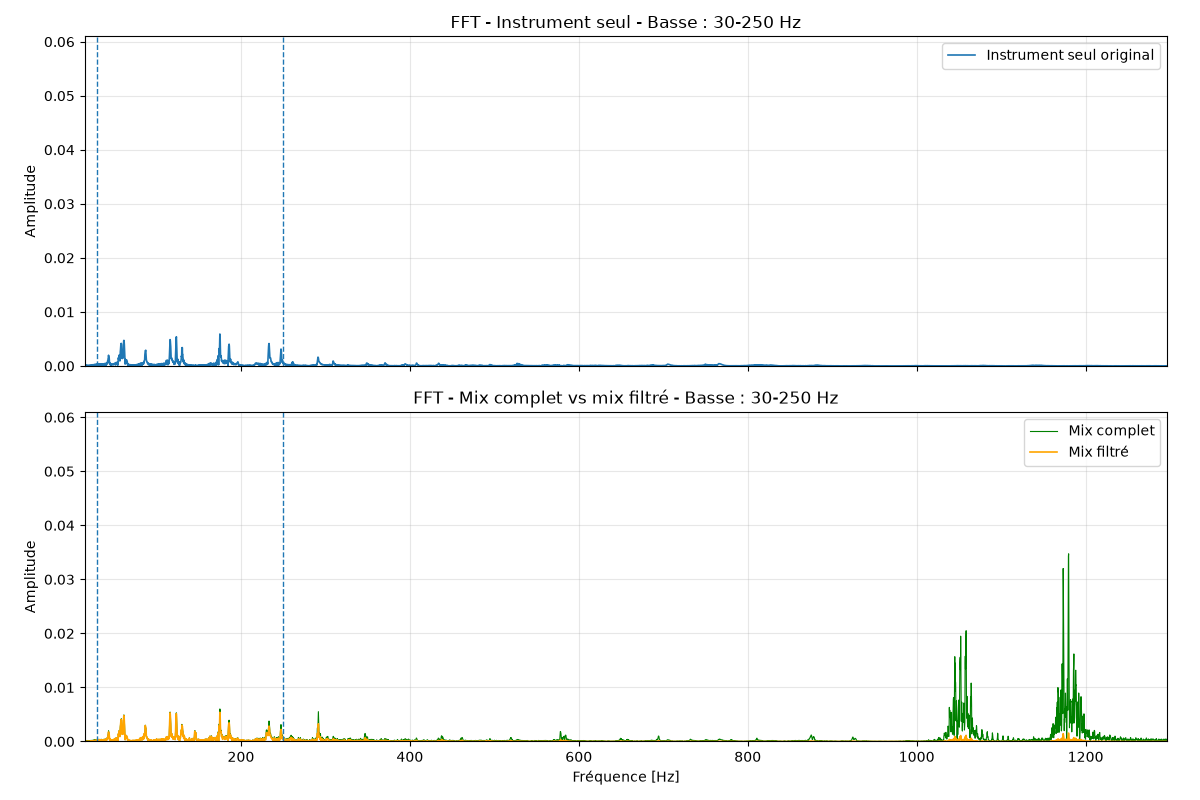
\includegraphics[width=0.75\textwidth]{img/bass_fft.png}
\end{figure}
    
\end{frame}

\subsection{Les anti-windups}

\begin{frame}{Utilité}
    \begin{block}{Explication}
        % Dans un contrôleur PID, le terme de l'intégral a pour rôle d'éliminer l'erreur statique en accumulant l'erreur au cours du temps. Cependant, lorsque l'actionneur atteint ses limites physiques de fonctionnement, la commande calculée par le contrôleur ne peut pas être appliquée intégralement. On parle alors de saturation.
        
        \begin{itemize}
            \item Utiliser le terme intégral du contrôleur PID.
            \item Éliminer l'erreur statique.
            \item Limiter les effets de la saturation.
        \end{itemize}
    \end{block}
    
    \begin{figure}
        \centering
        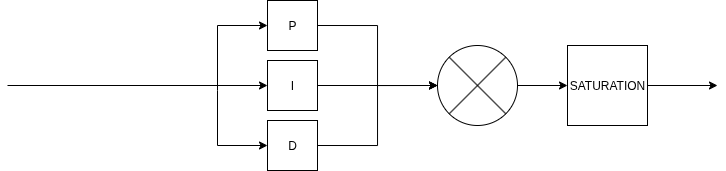
\includegraphics[width=0.8\textwidth]{img/PID.png}
    \end{figure}
    
    
\end{frame}

\begin{frame}{Représentation graphique}
    
    \begin{figure}
        \centering
        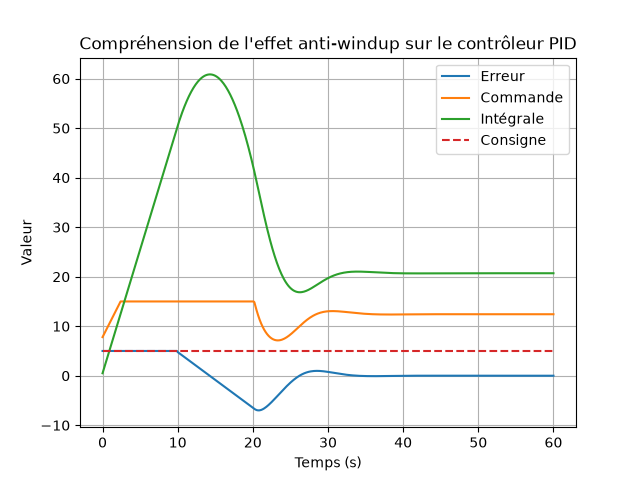
\includegraphics[width=0.65\textwidth]{img/integralWindup.png}
    \end{figure}
    
\end{frame}

\begin{frame}{Anti-windup clamp}
    \begin{block}{Explication}
        Bloque la valeur du terme intégral lorsqu'elle atteint une borne prédéfinie.
    \end{block}
    \begin{block}{Equation}
    $$
    I_{k} =
    \begin{cases}
        I_{max}, & \text{si } I_{k} > I_{max} \\
        I_{min}, & \text{si } I_{k} < I_{min} \\
        I_{k}, & \text{sinon}
    \end{cases}
    $$
    \end{block}
    
\end{frame}

\begin{frame}{Avantages et inconvénients}

    {
    \setbeamercolor{block title}{fg=white,bg=ufcgreen}
    
    \begin{block}{Avantages}
    % \begin{itemize}
    %     \item Simple à implémenter et à configurer
    %     \item Permet de limiter rapidement l'accumulation du terme intégral lors de la saturation
    %     \item Améliore la stabilité du système en évitant les dépassements excessifs
    % \end{itemize}
    \begin{itemize}
        \item Simplifier l'implémentation.
        \item Limiter l'accumulation du terme intégral en saturation.
        \item Réduire les dépassements du système.
    \end{itemize}
    \end{block}
    
    }
    
    
    \begin{block}{Inconvénients}
    % \begin{itemize}
    %     \item Difficulté de définir des bornes appropriées pour le terme intégral dans certains systèmes
    %     \item Ne pas être efficace dans les systèmes avec des dynamiques complexes
    % \end{itemize}
    
    \begin{itemize}
        \item Définir des bornes adaptées au terme intégral.
        \item Gérer les systèmes à dynamiques complexes.
    \end{itemize}
    \end{block}
\end{frame}

\begin{frame}{Anti-windup back-calculation}
    \begin{block}{Explication}
    Corrige progressivement l'intégrateur en fonction de l'écart entre la commande calculée par le PID et la commande réellement appliquée après la saturation.
    \end{block}
    
    \begin{block}{Equation}
    $$I_{k} = I_{k-1} + K_i e_{k} \Delta t + K_{aw} (u_{sat_k} - u_{k})$$
    
    où :
\begin{itemize}
    \item $K_{aw}$ est le gain de l'anti-windup. Souvent de la forme $\frac{1}{T_{t}}$, où $T_{t}$ est une constante de temps d'anti-windup réglée en fonction de la dynamique du système.
    \item $u_{k}$ est la commande calculée.
    \item $u_{sat_k}$ est la commande réellement envoyée à l'actionneur.
\end{itemize}
    \end{block}
\end{frame}

\begin{frame}{Avantages et inconvénients}

    {
    \setbeamercolor{block title}{fg=white,bg=ufcgreen}
    
    \begin{block}{Avantages}
    % \begin{itemize}
    %     \item Réduit fortement le dépassement
    %     \item Possède une récupération rapide après une saturation
    %     \item Plus fidèle au comportement réel de l'actionneur
    % \end{itemize}
    
    \begin{itemize}
        \item Réduire les dépassements.
        \item Améliorer la récupération après saturation.
        \item Représenter fidèlement le comportement de l'actionneur.
    \end{itemize}
    \end{block}
    }
    
    
    \begin{block}{Inconvénients}
    % \begin{itemize}
    %     \item Plus complexe à configurer
    %     \item Nécessite un réglage précis du gain $K_{aw}$ pour éviter les oscillations ou la dégradation de la stabilité
    % \end{itemize}
    \begin{itemize}
        \item Complexifier la configuration.
        \item Régler précisément le gain $K_{aw}$.
    \end{itemize}
    \end{block}
\end{frame}

\begin{frame}{Exemple drone}

    \begin{figure}
        \centering
        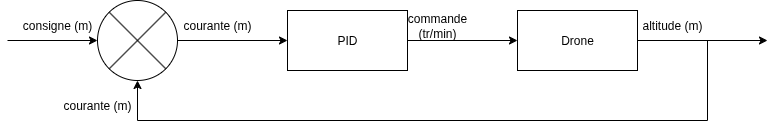
\includegraphics[width=\textwidth]{img/schema_drone.png}
    \end{figure}
    
    \vspace{-7mm}
    
    \begin{columns}[t]
    
        \begin{column}{0.48\textwidth}
        
            \begin{block}{Configuration}
                \begin{itemize}
                    \item Drone.
                    \item Contrôleur PID.
                    \item Temps de simulation 60 secondes.
                \end{itemize}
            \end{block}
        \end{column}
        
        \begin{column}{0.48\textwidth}
        
            \begin{block}{Objectifs}
                \begin{itemize}
                    \item Retenir le drone pendant 10 secondes.
                    \item Atteindre 5 mètres d'altitude en restant stable.
                    \item Utiliser les anti-windups clamp et back-calculation pour les comparer.
                \end{itemize}
            \end{block}
        \end{column}
    \end{columns}
    
    \begin{block}{Remarque}
    Contexte de simulation $\rightarrow$ résultats pas représentatifs de la réalité
    \end{block}

\end{frame}

\begin{frame}{Comparaison des méthodes}

\vspace{5mm}

\centering

\begin{tabular}{|l|c|c|c|}
\hline
&
\makecell{Altitude\\max. (m)} &
\makecell{Dépassement\\max. (\%)} &
\makecell{Temps de\\stabilisation\\$\pm5\%$ (s)} \\
\hline
Sans anti-windup & 12 & 140 & 32.2 \\
\hline
Clamp & 7.32 & 46 & 21.6 \\
\hline
Back-calculation & 5.31 & 6.2 & 18.9 \\
\hline
\end{tabular}

\end{frame}

\subsection{La chaîne de compilation}

\begin{frame}{Représentation}

    \begin{figure}
        \centering
        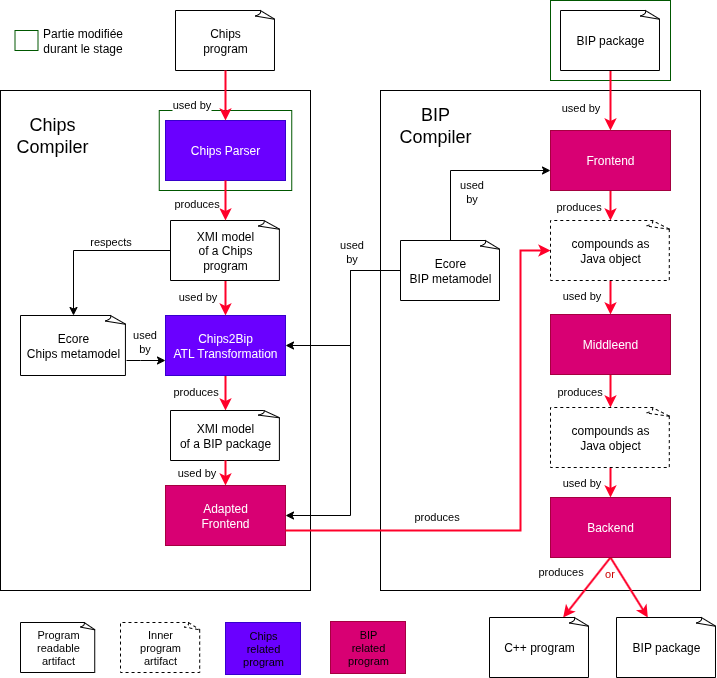
\includegraphics[width=0.5\textwidth]{img/architecture_partie_modifier.png}
    \end{figure}
    \vspace{-5mm}
    Démonstration
\end{frame}